\section{\textit{Estrutura}}

\subsection{Apresentação e Resumo}
    Desenvolvimento de uma plataforma física que acomode e dê suporte aos componentes dos sistemas de controle e energia, sistema eletrônico e também dos sistemas mecânicos que incluem o sistema de seleção de garrafas, triturador de plásticos, armazenamento das garrafas de vidros.

\subsection{Principais Características}

\subsubsection{Extrutura externa}
    A estrutura externa será composta por uma gaiola tubular que funcionará como armação  principal, envolvidos por placas de zinco. O aço AISI 1020 foi selecionado para os tubos quadrados de aço AISI 1020, que é amplamente utilizados para aplicações similares, além da confiabilidade, suas propriedades mecânicas atendem as necessidades do projeto. As placas de zinco foram escolhidas pois é um material de baixo e custo, além de ser um material de alta manuseabilidade, tornando o processo de fixação na armação principal mais fácil.

\subsubsection{Triturador}
    O triturador de plástico a ser utilizado neste projeto foi dimensionado e tomando como base trituradores disponíveis no mercado e projetos open source disponibilizados na internet. Após modelagem, as peças serão manufaturadas através de procedimentos de solda e de usinagem, onde estão incluídos o corte por jato d'água e torneamento. Idealmente algumas peças dos triturador o uso de aços inoxidáveis são necessários, visto que garrafas PET comumente possuem resíduos orgânicos. Todavia, para este projeto as peças usinadas serão de aço AISI 1020 ou AISI 1045, que possuem um custo financeiro inferior ao inoxidavel e que funcionarão de maneira satisfatória para o protótipo proposto.

\subsubsection{Mecanismo de pesagem e seleção de garrafas}
    O mecanismo de pesagem e seleção de garrafas a ser desenvolvido consiste em uma estrutura para a pesagem da garrafa e de um mecanismo que direciona cada tipo de garrafa a seu compartimento, seja ele o triturador ou as prateleiras de armazenamento de garrafas de vidro. A pesagem das garrafas será realizada através de uma célula de carga fixada e de uma base de apoio, para que as garrafas sejam pesadas corretamente. O mecanismo direcionador será do tipo mesa linear, que possui dois guias, um fuso e um motor de passo, permitindo o movimento em uma única direção.

\subsubsection{Compartimentos de armazenamento}
    O compartimento de armazenamento de plástico triturado será desenvolvido em madeira no formato de gaveta. Também em madeira, serão as canaletas do compartimento de armazenamento de vidro, que terão o intuito de guiar as garrafas até o fundo do compartimento. Para tal, as canaletas possuirão uma angulação e batentes. Haverá uma porta de acesso para o recolhimento dos resíduos e de limpeza dos compartimentos.

\subsection{Testes}

    Realização de diversos testes para garantia do correto funcionamento da máquina como um todo.

\begin{itemize}
\item Teste para tempo médio de trituração do plástico. 
\item Experimentos para avaliar a eficácia do armazenamento das garrafas de vidro.
\item Testes de tempo de seleção das garrafas.
\item Análises computacionais, utilizando CATIA V5 ou ANSYS 18.1, para validação do design e da estrutura, de forma a garantir correta integração entre os sistemas e correto dimensionamento para suportar os esforços e vibrações existentes no projeto.
\end{itemize}

\section{\textit{Sistema de Controle de Energia e Segurança}}

\subsection{Apresentação e Resumo}

    O subsistema de energia irá dimensionar o motor elétrico que será utilizado na máquina, assegurará o sistema de proteção da mesma e também o sistema de emergência. Ele estará integrado com o subsistema de estrutura interna, realizando o acionamento do motor elétrico, juntamente com o subsistema da eletrônica, para o funcionamento do triturador.

\subsection{Principais Características}

    O triturador  da  máquina será movido através de um motor elétrico, que terá o controle de sua velocidade a partir de um redutor, equipamento mecânico que tem como função principal a redução da rotação de um acionador. O motor receberá sinal do subsistema da eletrônica e então, por partida direta será acionado, devendo manter aproximadamente 70 rotações por minuto.

    Pelo fato do motor elétrico ter grande importância no equipamento, será necessário uma proteção contra possível sobrecarga, diante disso o relé térmico entra em funcionamento, sendo responsável por proteger o motor de possíveis irregularidades, como o sobreaquecimento do motor elétrico. Além disso, será construído um sistema de proteção dos circuitos eletrônicos da máquina, a partir da montagem de um quadro com fusível e disjuntor. Por fim, teremos o sistema de emergência, que poderá interromper o funcionamento da máquina quando necessário, por meio de uma chave/botão.

\subsection{Testes}

    Para a validação do subsistema de alimentação alguns testes deverão ser realizados:

\begin{itemize}
\item Teste contínuo do sistema de emergência da máquina.
\item Teste de acionamento do motor elétrico.
\item Teste do controle de rotação do motor.
\item Teste de acionamento do motor com os subsistemas da máquina.
\item Teste de proteção elétrica.
\end{itemize}

\section{\textit{Sistema Eletrônico}}

\subsection{Apresentação e Resumo}

    O sistema eletrônico do projeto em questão estará presente nos subsistemas de separação de garrafas, interação máquina-usuário e acionamento do triturador. Serão utilizados componentes como microprocessadores, microcontroladores, sensores e motores elétricos. O funcionamento dos subsistemas será descrito no subtópico seguinte.

\subsection{Principais Características}

    Primeiramente, no subsistema de separação de garrafas, existirá a etapa de reconhecimento através de leitura de QR Code/Barcode (á definir), que estará presente nas garrafas a serem reaproveitadas, dos parâmetros relevantes para a preparação de reciclagem, tais como tipo de material da garrafa, peso médio, e para qual tratamento de preparação para reciclagem o material deve ser encaminhado. O sistema será gerido, de forma geral, através de um microprocessador Raspberry Pi 3.

    O sistema irá acionar o controle de abertura e fechamento de um compartimento para que o usuário insira a garrafa a ser reciclada, através do acionamento de um servo motor controlado através de um microcontrolador ESP8266.

    Em seguida, ocorrerá a confirmação do tipo da garrafa e se a mesma está cheia ou vazia através de seu peso, além de uma possível nova confirmação do tipo de material da garrafa através de sensores, com todos os dados contidos no código lido anteriormente na garrafa, comparadas as informações contidas no banco de dados.  Estas confirmações serão realizadas através de uma célula de carga e possivelmente um sensor capacitivo de presença. Caso haja alguma não-conformidade na garrafa inserida, o compartimento onde a garrafa foi inserida será aberto novamente, indicando a retirada da garrafa.

    Após validada a garrafa inserida pelo usuário, a mesma será direcionada para o tratamento ideal, de acordo com o seu material de composição. Direcionamento este feito através de um trilho com movimentação baseada em um motor de passo. Caso a garrafa seja de plástico, a mesma será movida para o lado em que se possui o subsistema de trituração. Caso seja de vidro, a garrafa será movida para o lado que possui canaletas para armazenamento.  A capacidade de armazenamento será monitorada através de software e um sensor de presença (capacitivo ou infravermelho).

    Além do subsistema de separação de garrafas, o sistema eletrônico engloba também a parte de interação maquina-usuário. Inicialmente, através de leitura de QR code gerado pelo aplicativo e em seguida. Através de um display para exibir informações relevantes ao usuário, como por exemplo, nome do usuário e status de operação da máquina, acompanhado de confirmações sonoras. Para isso, o sistema se utilizará também do microprocessador Raspberry Pi 3, além de um display LCD 16x2 e um buzzer sonoro.

\subsection{Testes}

    Uma série de testes deverão ser realizados para validação dos subsistemas, testes como:

\begin{itemize}
\item Testes de adequação de célula de carga em seu uso específico, calibração da célula de carga via software.
\item Testes de adequação dos sensores capacitivos para reconhecimento de materiais.
\item Testes de segurança relacionados à tensões e correntes totais dos componentes.
\item Testes para definir ponto de partida e parada do motor de passo.
\item Testes para verificar o funcionamento e definir se será utilizado QR code ou barcode para identificação da garrafa.
\end{itemize}

\section{\textit{Interação com o usuário}}

\subsection{Apresentação e Resumo}
    O subsistema de software será responsável pelo desenvolvimento de uma interface usuário-máquina em um smartphone capaz de se comunicar efetivamente com a máquina de separação de garrafas, persistir os dados de usuário em tempo real, e garantir conexão através da leitura de um QR Code gerado pelo próprio dispositivo móvel. Para alcançar os objetivos e os requisitos elicitados, existem dois fluxos representados no seguinte diagrama: 

\begin{figure}[!ht]
	\centering
		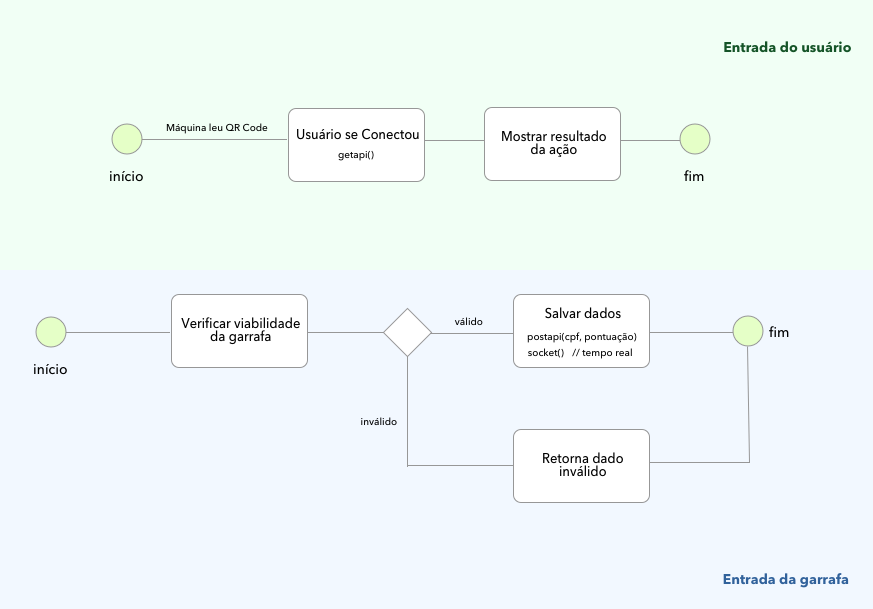
\includegraphics[scale=0.5]{figuras/representacao}
	\caption{Diagram do fluxo de interação entre máquina e usuário.}
\end{figure}

\subsection{Principais Características}

\subsubsection{Pré-uso}
    Antes da utilização efetiva da troca de garrafas no aplicativo desenvolvido, o usuário irá precisar se cadastrar no sistema de forma simples, com informações como seu nome e cpf. Com o login criado, e o usuário logado, o sistema será capaz, quando solicitado, de gerar um QR Code onde a máquina de separação de garrafa pode fazer a leitura e começar o fluxo principal do subsistema.

\subsubsection{Entrada de Usuário}
    A entrada do usuário representa a conexão entre o dispositivo móvel do usuário, com a máquina de separação de garrafas. Para iniciar todo o fluxo, o usuário clica em um botão de gerar o QR Code, e ao aproximar de um leitor da máquina, os dados do usuário serão transmitidos para a máquina. Sendo assim, a máquina consegue criar a sessão necessária para outros subsistemas agirem. O resultado dessa leitura será mostrada na máquina, seja um erro na conexão, ou o nome do usuário ali representado.

\subsubsection{Entrada da Garrafa}
    Com a sessão devidamente inicializada, a garrafa poderá ser inserida na máquina. Sendo assim, ao inserir a garrafa, a leitura de seu código de barras será feita, e o software será capaz de analisar a viabilidade da garrafa. No caso de inserção de uma garrafa viável, o software terá implementação de uma socket, comunicando em tempo real com um banco de dados na nuvem que irá salvar os dados, contabilizar sua pontuação, atualizar a pontuação na tela do aplicativo do usuário, e registrar os dados de forma segura e sem exclusão. 

    Caso a inserção dê uma garrafa inviável, a mesma comunicação em tempo real irá acontecer, conseguindo transmitir aos outros subsistemas o dado inválido. Vários fluxos de entrada de garrafa poderão feitas.

\subsubsection{Arquitetura}
    A arquitetura de software é a estrutura do sistema, a qual é composta de elementos de software, das propriedades externamente visíveis desses elementos, e dos relacionamentos entre eles; é a abstração do sistema (Bass, 2003). 

    Com o aumento da complexidade das aplicações desenvolvidas torna-se fundamental a separação entre os dados (Model) e o layout (View). Desta forma, alterações feitas no layout não afetam a manipulação de dados, e estes poderão ser reorganizados sem alterar o layout. Como o software que controlará e se comunicará com a máquina de separação de garrafas será desenvolvida em cima de um aplicativo mobile, iremos utilizar a framework Quasar CLI, construída em cima do Vue, outra framework em Javascript, para desenvolver todo o aplicativo. Sua arquitetura é baseada no MVVM (Model-View-ViewModel), representada na imagem abaixo.

\begin{figure}[!ht]
	\centering
		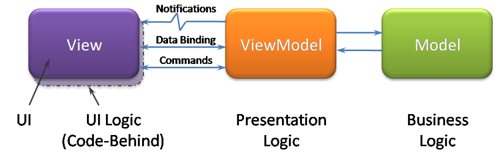
\includegraphics[scale=1]{figuras/mvvm}
	\caption{Modelo arquitetural MVVM.}
\end{figure}

    A camada Model (Modelo) não conhece a View (Camada de apresentação) e vice-versa, na verdade a View conhece a ViewModel e se comunica com ela através do mecanismo de binding. E são os avançados mecanismos de binding, eventos roteados e comandos roteados, que fazem do MVVM um pattern poderoso para construção da aplicação necessária.

    Já o socket formalmente falando é forma de permitir que dois processos se comuniquem (Inter-process communication). Esses processos podem ou não estar na mesma máquina. A imagem abaixo ilustra a troca de informações em tempo real da API do socket.

\begin{figure}[!ht]
	\centering
		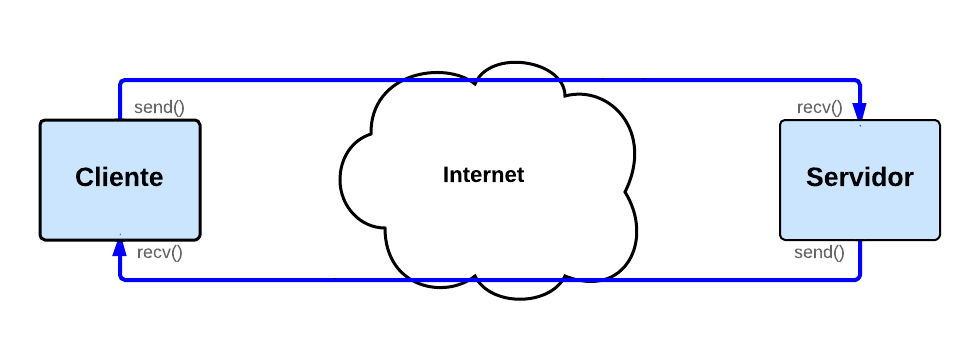
\includegraphics[scale=0.5]{figuras/socket}
	\caption{Diagrama de funcionamento de um WebSocket.}
\end{figure}

\subsection{Prototipação e Testes}

    Antes do começo da primeira sprint de desenvolvimento, uma fase de prototipação do aplicativo será feito em cima de princípios de design thinking e Lean Startup para obtenção das funcionalidades em forma visual.

    Já durante o desenvolvimento, serão desenvolvidos testes unitários para agregar e medir qualidade no código gerado. A API desenvolvida, a persistência dos dados, e a comunicação em tempo real serão testados e relatados Quanto ao aplicativo que cuidará da interface usuário-máquina, testes e2e serão feitos no que tange ao QR Code, login e cadastro de usuário, e tudo que entra no fluxo do front-end.

	Como será utilizado um processo ágil de desenvolvimento de software, as sprints terão obrigatoriedade de constituir testes, e de acordo com sua cobertura e resultados obtidos, decisões ao longo do projeto devem ser tomados. Os testes serão feitos de acordo com cronograma disposto.

\subsection{Observações importantes}

\begin{table}[!ht]
\centering
\caption{Tabela de observações importantes}
\label{my-label}
\begin{tabular}{|l|l|}
\hline
\textbf{Descrição}                                                                                                                                                                & \textbf{Motivo}                                                                                                            \\ \hline
\begin{tabular}[c]{@{}l@{}}Versionamento será na plataforma \\ GitHub, e será disponibilizado para todos os\\ membros da equipe\end{tabular}                                      & Acessibilidade e projeto público                                                                                           \\ \hline
\begin{tabular}[c]{@{}l@{}}O backlog de todo o projeto será feito logo\\ após a aprovação da prototipação\end{tabular}                                                            & \begin{tabular}[c]{@{}l@{}}Alinhamento dos requisitos e riscos do\\ projeto junto aos objetivos do subsistema\end{tabular} \\ \hline
As sprint serão semanais                                                                                                                                                          & Imersão, produtividade                                                                                                     \\ \hline
\begin{tabular}[c]{@{}l@{}}A parte de comunicação entre os módulos de\\ comunicação será desenvolvida pela equipe\\ de eletrônica conjunto a equipe de software\end{tabular} & Tecnologias convergentes                                                                                                   \\ \hline
\end{tabular}
\end{table}
